\section{Architectural considerations}
\label{sec:architecture}

	\subsection{Separation of concerns}
	\label{sec:separation-conceprns}
	
	The successful application of an ontology or the development of an ontology-based system depends not just on building a good ontology but also on fitting this into an appropriate development  process.  All computing information models suffer from a semantic schizophrenia. On the one hand, the model represents the domain; on the other hand, it represents the implemented system, which then represents the domain. These different representation requirements place different demands upon its structure \cite{partridge2013}.
	
	One of the common ways to manage this problem is a separation of concerns. OMG's Model Driven Architecture (MDA) \cite{mda-paper} is a well documented structure where a model is built for each concern and this is transformed into a different model for a different concern. 
	
	\textit{Transformation} deals with producing different models, viewpoints, or artefacts from a model based on a transformation pattern. In general, transformation can be used to produce one representation from another, or to cross levels of abstraction or architectural layers \cite{mda-guide2}. 
	
	The process described in Section \ref{sec:process-approach} adopted some of these principle and employs model transformation to achieve the project objectives.

	\subsection{Semantics}
	\label{sec:semantics}
	
	Users of OWL \citep{owl2} can actually select between two slightly different semantics: \textit{direct semantics} that corresponds to the Description Logics (DL) \cite{dl-baader2004description}, and \textit{RDF-based semantics} that is based on translation of the OWL axioms into directed graphs. In this document we assume by default the direct semantics. In particular cases (i.e. SPARQL entailments and SHACL data shapes) RDF-based semantics is adopted and is explicitly mentioned in the document. 
	
	Description logics provide a concise language for OWL axioms and expressions. DLs are characterised by their expressive features. The description logic that supports all class expressions with $>, \bot, \sqcap, \sqcup, \neg, \exists$ and $\forall$ is known as $\mathcal{ALC}$ (which originally used to be an abbreviation for Attribute Language with Complement). For a formal introduction into DL please consult \citet{dl-baader2004description}.
	
	Inverse properties are not supported by $\mathcal{ALC}$, and the DL we have introduced above is actually called $\mathcal{ALCI}$ (for $\mathcal{ALC}$ with inverses) \cite{krotzsch2012owl}. Many description logics can be defined by simply listing their supported features. We will use this notation when discussing degrees of expressivity for the ontology layers in Section \ref{sec:expressivity}.
	
	Computing all interesting logical conclusions of an OWL ontology can be a challenging problem, and reasoning is typically multi-exponential or even undecidable. To address this problem, the recent update OWL 2 of the W3C standard \citep{owl2.0,owl2} introduced three profiles: \textit{OWL EL}, \textit{OWL RL}, and \textit{OWL QL}. These lightweight sublanguages of OWL restrict the available modelling features in order to simplify reasoning. This has led to large improvements in performance and scalability, which has made the OWL 2 profiles very attractive for practitioners \citep{krotzsch2012owl}.
	
	On the other hand, the validation data shapes are expressed using Shapes Constraint Language (SHACL) \cite{shacl-spec}. Its semantics is based on RDF graphs but full RDFS inferencing is not required. SHACL processors may operate on RDF graphs that include RDF entailments \citep{rdf11-semantics} and SPARQL specific entailments \citep{sparql11-entailment}. The entailment regime specifies conditions that address the fourth condition on extensions of basic graph pattern matching \citep{rdf-semantics,rdf11-semantics}. 
	
	This architecture delimits different concerns in Section \ref{sec:layers} in a stack of layers and assigns levels of expressivity to each of the layers in Section \ref{sec:expressivity}.
	
	\subsection{Open/Closed world assumptions}
	\label{sec:world-assumption}
	

	

	
	\subsection{Layers and components}
	\label{sec:layers-components}
	
	This architecture is organised in \textit{horizontal layers} and vertically slicing \textit{components}. The \textit{components} reflect the organisation of the formal ontology based on a logical content division of the UML conceptual model into packages and modules. This division increases the maintainability of entire content. The models and their components are not disconnected from one another. The relations between them are represented in Figure \ref{fig:components} where each component is represented as an UML package. The conceptual model serves as the single source of truth, from which the three components of the formal model are derived. Each of these components can be further divided into modules. 
	
	The main ontology packages are: the \textit{core ontology}, \textit{data shapes}, and \textit{formal ontology restrictions}. The these formal modules are derived from the conceptual model through model transformations as described in Section \ref{sec:process-approach} following the rules laid out in \citet{costetchi2020c}.
	
	The \textit{core ontology} is the foundational, and serves as a backbone for the other components. It establishes the identifiers and the basic definitions of classes and properties.
	 	
	The \textit{data shapes} represent constraints on how the core ontology can be instantiated and the set of controlled value lists associated to it. 	
	
	The \textit{formal ontology restrictions} cover intensional class and property definitions used for deriving additional knowledge from factual information. Both, the data shapes and the ontology restrictions are defined as extensions that are flashing out the core ontology which plays, in this case the role of a backbone.
	
	\begin{figure}[!ht]
		\centering
		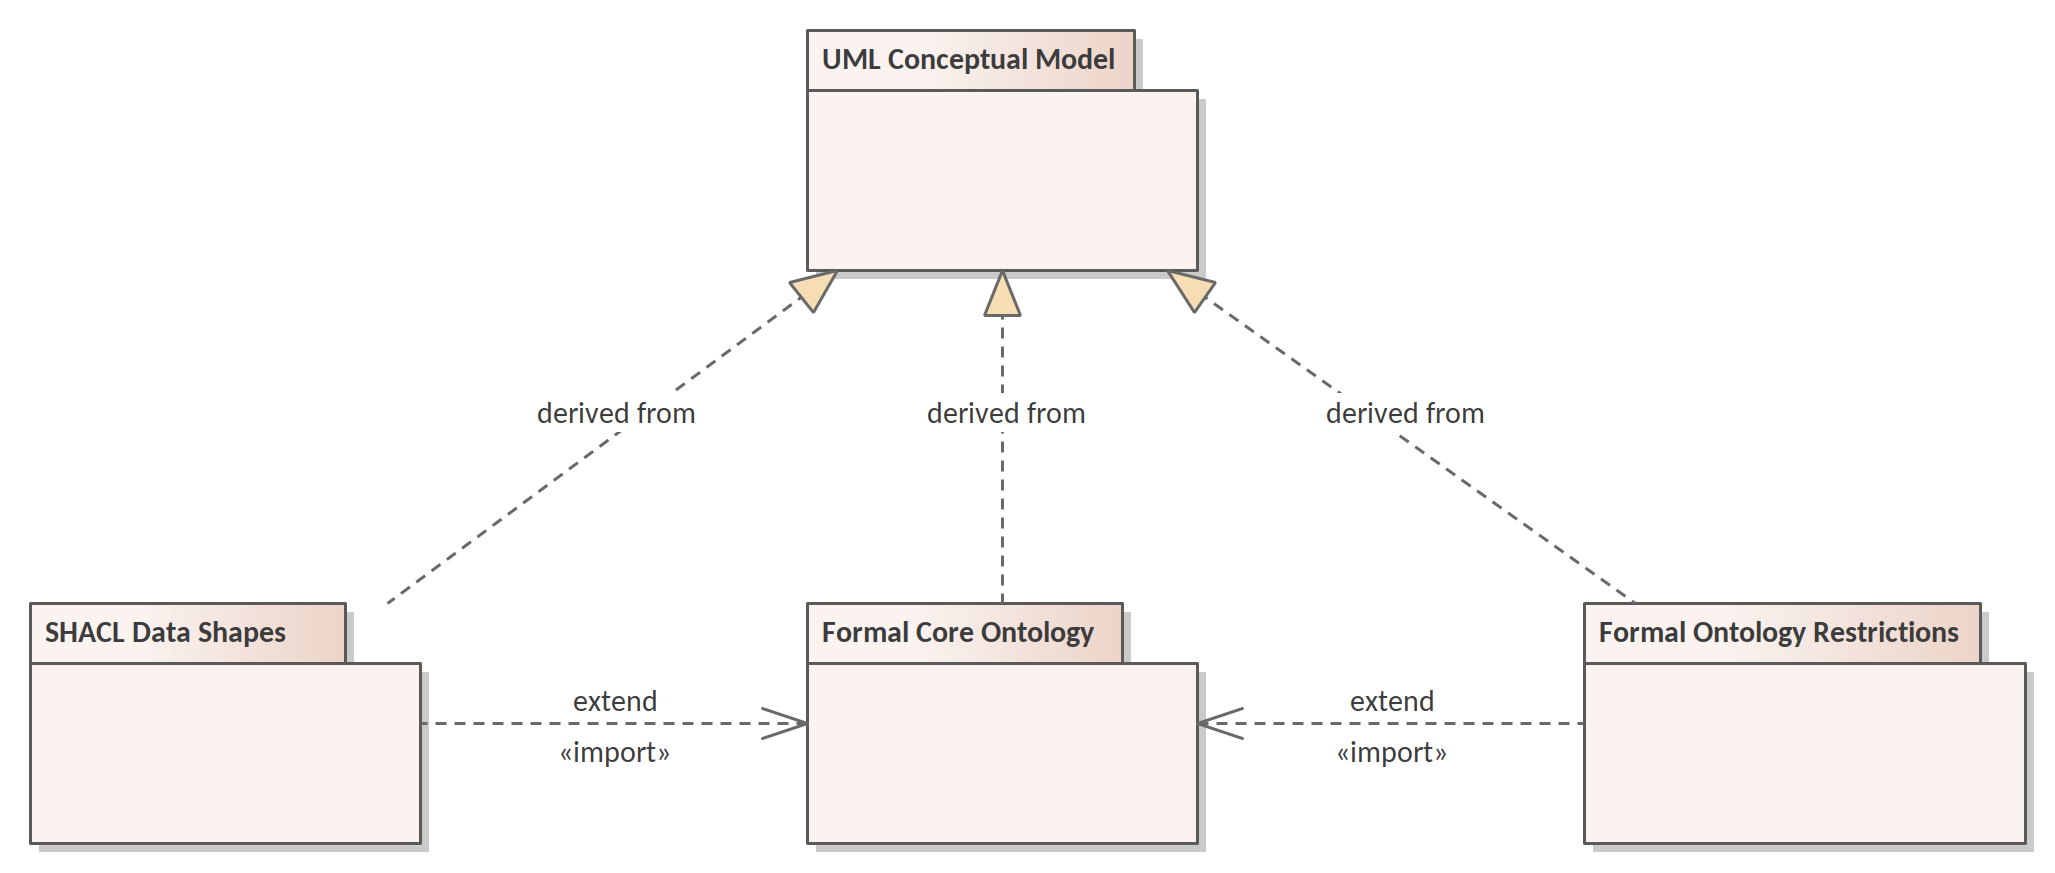
\includegraphics[width=0.99\textwidth]{../img/uml.png}
		\caption{The main components of the eProcurement ontology and their relation to each other and the UML conceptual model}
		\label{fig:components}
	\end{figure}
	
	This architecture distinguishes the following layers: the \textit{conceptual layer}, \textit{core definition layer}, \textit{validation layer} and \textit{reasoning layer}. These \textit{layers} can be though of as formal languages with well defined boundaries and extents. The diagram in Figure \ref{fig:layers} presents the organisation the ontology layers along two axes: \textit{expressivity} and \textit{detail}. 
	
	The \textit{expressivity} of a language is the breadth of ideas that can be represented and communicated in that language. The more expressive a language is, the greater the variety and quantity of ideas it can be used to represent. The design of a language and its formalism involves an inevitable trade-off between the expressive power and its ``analyzability'', which translates directly into computation difficulty. The more a formalism can express, the harder it becomes to understand, i.e. compute, what do instances of it mean.
	
	The \textit{detail} refers to how much description and aspects of the domain concepts are considered. This dimension is plays a pragmatic rather than formal role. The rationale is that lower level of detail is useful and re-usable to a wider public, but for a set of relatively simple tasks. As the level of detail increases, the difficulty to operate on it also increases thus the user base shrinks and the task complexity rises. 
	
	The detail axis starts, on one side, from establishing the concepts identity, labels, natural language  definitions; continues through establishing relations and constraints; and ends, on the other side, with formulating special logical conditions, implications and inference rules.
	
	\begin{figure}[!ht]
		\centering
		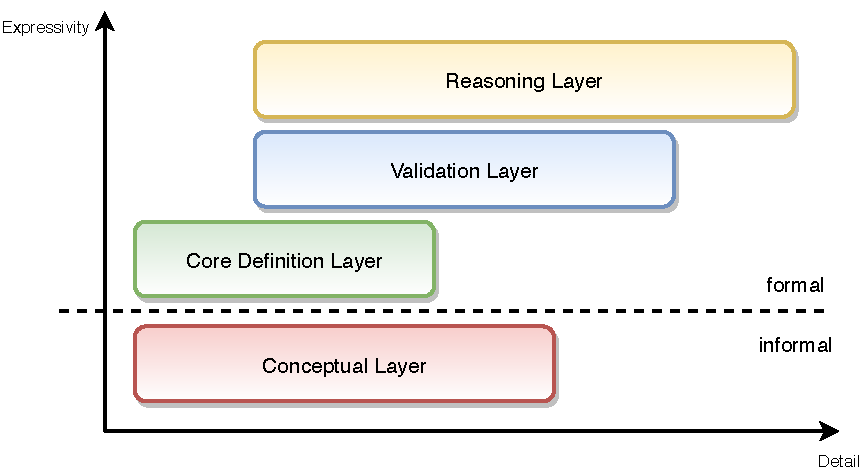
\includegraphics[width=0.9\textwidth]{../img/eProcurement-layers}
		\caption{Expressivity and extent of the eProcurement ontology layers}
		\label{fig:layers}
	\end{figure}
	
	The \textit{conceptual layer} accommodates informal representation of the business objects, places, things, actors in the ``real world'' not representations of these things in the information system. It is situated at the base of the diagram with lowest expressivity because it has not formal semantics but with a wide coverage of detail. The dotted line delimits the border between formal and informal layers.
	
	In the conceptual layer is situated the \textit{UML conceptual model}, which is described in Section \ref{sec:uml-model}. This model is also called \textit{computation independent model} because it is informal and its main purpose is to interface the domain experts with an explicit conceptual representation of the domain.
		
	In the formal section of the diagram, the expert knowledge is expressed using descriptive languages with a formal semantics (see Section \ref{sec:semantics}), which in this architecture are primarily OWL 2\cite{owl2} and SHACL\cite{shacl-spec}. 
		
	The \textit{core layer}, is situated the core ontology, which has as a primary goal to define the main concepts and relations of the ontology. It is limited to the declarative axioms of the ontology and therefore serves primarily for vocabulary and identity establishment. For this reason it is represented as having the lowest formal expressivity and the lightest level of detail in comparison to other layers. It plays the role of a backbone which is flashed out by other layers. 

	The \textit{validation layer} accommodates declarations of data shapes which represent constraints on the instance data, i.e. the ABox (see Section \ref{sec:model-data}). The assertions in this layer are interpreted done under the closed world assumption, making it possible to support validation functionality. The SHACL shapes are situated in this layer and are addressed in detail in Section \ref{sec:shapes}.
	
	The validation layer is situated immediately above the core definitions, being more expressive but also extending it with additional detail. Therefore it is shifted, on the detail axis, to the right towards more detail and leaving out the simple axioms as they are already covered in the core later.
	
	The \textit{reasoning layer} accommodates formal intensional definitions of the classes and properties. It is mostly formed of subclass restrictions and complex class definitions, and as well, domain and range specifications for properties. This layer provides assertions necessary to supports reasoning functionalities for eProcurement ontology. The formal ontology restrictions component is situated in this layer and is described in Section \ref{sec:restrictions}.
	
	Just like in the case of restrictions layer, the reasoning layer extends the core layer with higher level of detail and comprising assertions with higher expressive power. Therefore the simple details rest in the core layer permitting this one to focus on other ones. For this reason it is depicted as shifted to the towards the right side of detail axis.
	

	\subsection{Relationship between the model and data}
	\label{sec:model-data}
	
	DL ontologies are structured into two sets: \textit{ABox} and \textit{TBox}. The \textit{ABox} consists of all (class or property) instance assertions. The \textit{TBox }consists of all terminological axioms, i.e., of all subclass inclusion axioms. The ABox provides information about concrete individuals while the TBox describes general rules that hold for all individuals. In consequence, ABoxes tend to be much larger than TBoxes \citep{krotzsch2012owl}. In Figure \ref{fig:abox-tbox} is depicted the delimitation and relations between the TBox and box ABox components of the eProcurement ontology.
	
	\begin{figure}[!ht]
		\centering
		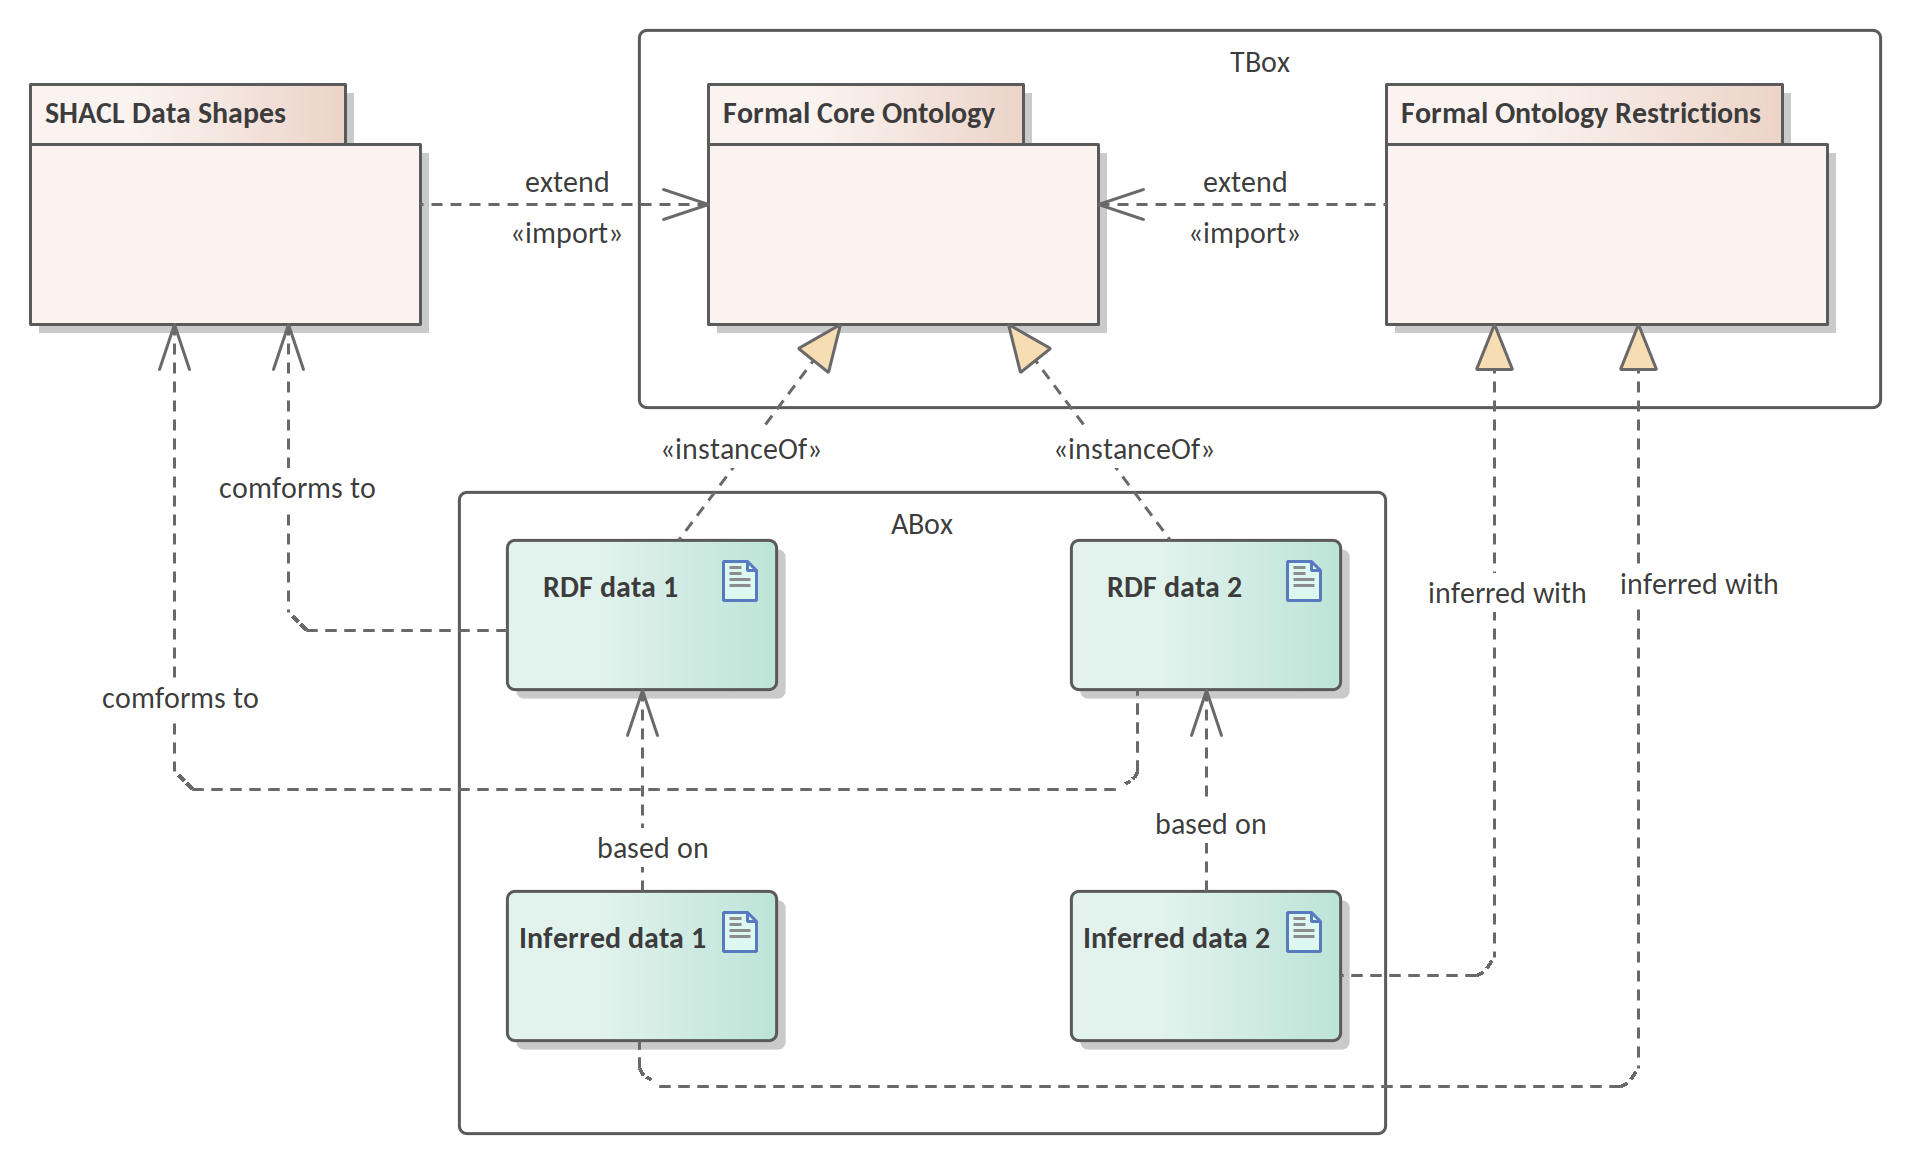
\includegraphics[width=0.99\textwidth]{../img/ontology.png}
		\caption{The relationship between the data and each of the ontology components}
		\label{fig:abox-tbox}
	\end{figure}
	
	To explain the relevance of each component, in Figure \ref{fig:abox-tbox}, two arbitrary datasets are brought as examples. They instantiate the core ontology, which means that they comprise of factual statements of concrete entities of eProcurement classes. In order to ensure that the instance data follow minimally the intended ontology design they need to comply with a set of data shapes. Once this condition is satisfied, then, new knowledge can be inferred from the provided facts, given the domain inference rules. The new knowledge is mainly oriented to solve the classification task and does not cover other types of inference. 	
	
	It is important to note that the data shapes fall out of the TBox as they serve the validation function and are based on a different set of assumptions. First they are interpreted under the closed world assumption, like in XML  or RDBM contexts (see Section \ref{sec:world-assumption}). Second they follow a RDF graph based semantics \ref{sec:semantics}.
	Next, each of these components is detailed in the sections below.
	
	\subsection{UML conceptual model}
	\label{sec:uml-model}
	
	
	
	\subsection{SHACL shapes}
	\label{sec:shapes}
	
	Application profiles represent a set of constraints on the logical model tying it to a particular system implementation. The application profiles, in this project, must be expressed using SHACL language [ref shacl spec]. The application profiles are extending the (core) formal model and can be derived from the conceptual model through transformation, or can be designed directly in the formal representation. 
	
	\subsection{Formal ontology restrictions}
	\label{sec:restrictions}
	
	%	In a formal system of logic used for knowledge representation, the open-world assumption is the assumption that the truth value of a statement may be true irrespective of whether or not it is known to be true. It is the opposite of the closed-world assumption, which holds that any statement that is true is also known to be true [Wikipedia].